\documentclass[11pt]{amsart}
\usepackage{geometry}                % See geometry.pdf to learn the layout options. There are lots.
\geometry{letterpaper}                   % ... or a4paper or a5paper or ... 
%\geometry{landscape}                % Activate for for rotated page geometry
%\usepackage[parfill]{parskip}    % Activate to begin paragraphs with an empty line rather than an indent
\usepackage{graphicx}
\usepackage{amssymb}
\usepackage{epstopdf}
\usepackage [autostyle, english = american]{csquotes}
\usepackage{hyperref}
\MakeOuterQuote{"}
\DeclareGraphicsRule{.tif}{png}{.png}{`convert #1 `dirname #1`/`basename #1 .tif`.png}

\title{Project 5: Deriving the Equilibrium Energy of an Ideal Gas using Markov Chains}
%\author{Jessica Bartley}
%\date{}                                           % Activate to display a given date or no date

\begin{document}
\maketitle
%\section{}
%\subsection{}

We start this project off by imagining a cube of arbitrary volume that is filled with an ideal gas.  This gas has thermodynamic properties described mathematically by the so-called Boltzmann distribution, 

\begin{equation}
P(q_i,p_i)=e^{-\beta H}
\end{equation}
\vspace{2 mm}

where $H$ is the total energy of the gas (the Hamiltonian) and $\beta = \frac{1}{kT}$, where $k$ is Boltzmann's constant with value $1.38 \times 10^{-23}$ $\frac{m^2 \cdot kg}{s^2 \cdot K}$, and $T$ is the temperature of an external reservoir in which the cube sits and is in thermal equilibrium with.  For our code we can normalize this $\beta$ to any value we choose.  In the template code (for whatever reason) $\beta = 4$, so we'll use that too.  We are going to use the Boltzmann distribution to simulate how gas molecules move over time.  We will use this information to find the energy of the gas as a function of time.  The resulting graph should appear as something like the attached graph, Figure 2 on final page.
\newline

The setup is relatively simple: imagine we start of with the (extremely improbable) event that all of the $N$ gas molecules are located at the exact same location at the bottom middle of the cube, Fig 1.  In the field of atomic molecular optics we would call this a "condensate."  Condensates only happens when the system has been forced into such a low energy state that the molecules collapse into each other.  Needless to say, our initial condensate does not want to stay in this configuration.  We wish to simulate what happens to the gas after we let it go free.  Intuition correctly tells us that the gas molecules disperse about the volume of the box.  We will program a series of Markov chains that simulate this dispersion process.
\newline

\begin{figure}[ht!]
\centering
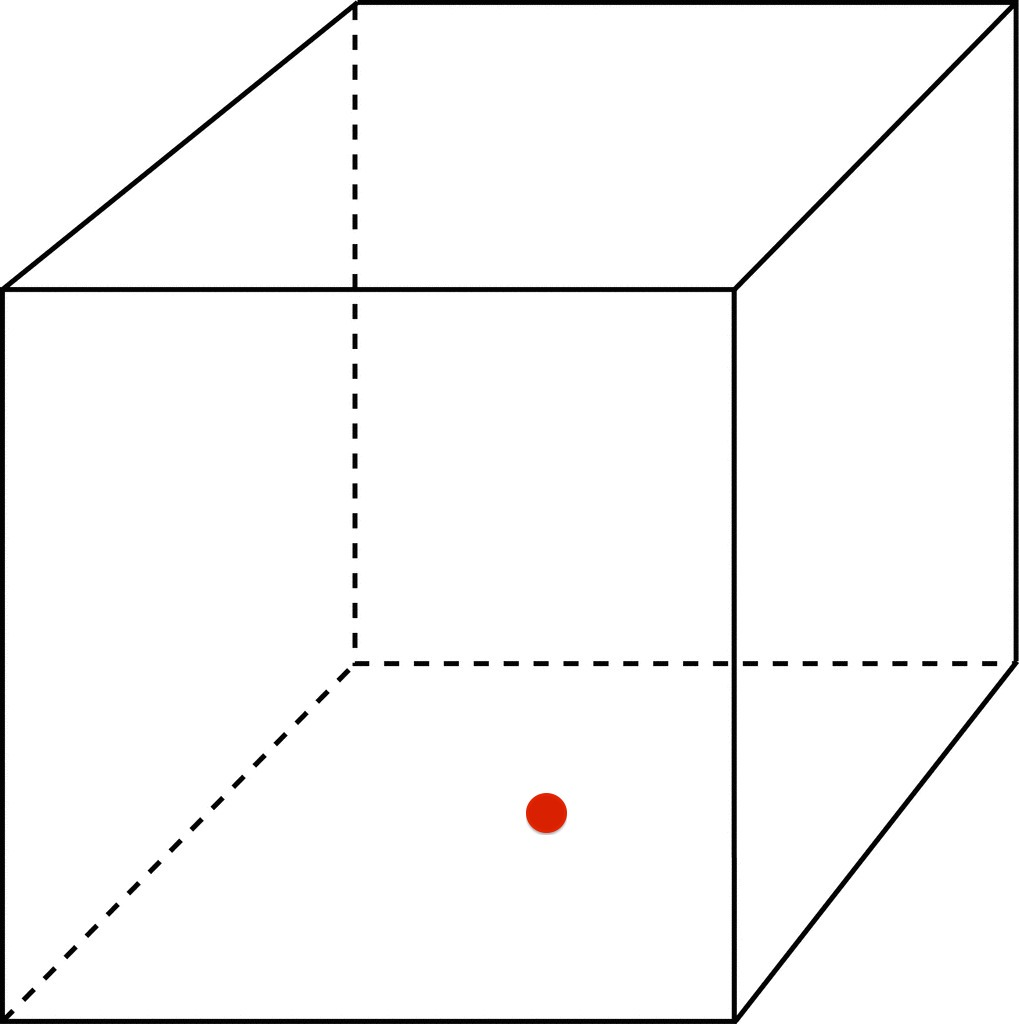
\includegraphics[width=40mm]{cube.jpg}
\caption{An initial condensate gas}
\label{overflow}
\end{figure}

\vspace{3 mm}

First we need to establish the initial conditions for the gas.  This will be an 6 $\times$ $N$ array of numbers where the 6 rows contain three spatial positions $q_1$, $q_2$, and $q_3$ and the three momenta $p_1$, $p_2$, and $p_3$.  These six coordinates fully describe the state of any given particle.  Initially this array will have all positions = $(0.5,0.5,0)$ and all momenta = 0.  We will change this array, or "ensemble", one column at a time until the entire array has changed.  Then, once all columns have been changed, we will repeat the process until the energy associated with each ensemble stabilizes to an equilibrium value.  This process is called a "Markov chain."  At any stage, the total energy of the gas is given by

\begin{equation}
H = \sum\limits_{i=1}^N \frac{1}{2} (p_{1,i}^2+p_{2,i}^2+p_{3,i}^2) + q_{3,i}
\end{equation}
\vspace{2 mm}

We will print out these ensemble energies after all columns have been cycled through.  The energy should ultimately stabilize after many iterations of ensembles.  To get to this equilibrium state we will have to loop over all particles (one sweep) and then loop over all ensembles ($M$ sweeps).
\vspace{2 mm}

What we need to do:
\begin{enumerate}
\item Establish the initial ensemble array.
\item Generate a trial configuration by randomly varying the position and momenta of $i$th particle in a loop from $i=1...N$: $q_i(trial)=q_i(current)+(X-0.5) \cdot \epsilon$ and $p_i(trial)=p_i(current)+(X-0.5) \cdot \epsilon$.  Here $X$ is a random number generated between 1 and 0, and $\epsilon$ is an arbitrarily small value.

\item We then check if the trial position and momenta are energetically favorable for the system.  That is, is the trial configuration more probable than the current configuration?  If the Boltzmann distribution $P(q_i,p_i)$ associated with the trial configuration is greater than the $P(q_i,p_i)$ for the previous configuration then, yes, the trial configuration is energetically favorable.  So, if $P(trial) \geq P(current)$ then we replace the current column with the trial column and go to step 2.  If $P(trial) < P(current)$ then we move to step 4.

\item It is possible, even if a trial configuration is not energetically favorable, that it might still randomly occur.  To account for this we calculate the probability of the energetically unfavorable event randomly occurring. The random event will occur if 

 \[
 \frac {P(current)}{P(trial)} \geq Y
\]

Where Y is a random number between 0 and 1.  Note, by nature of the Boltzmann probability, this ratio $ \frac {P(current)}{P(trial)}$ will always have a values between 0 and 1.  If this statement has a true value then we accept the trial configuration and replace the column.  If the ratio is less than the random number then we reject it and move on to the next particle (back to step 2).  This loop continues until we sweep over all particles.

\item After a complete sweep over all particles in the ensemble we calculate the energy of the gas via Equation 2.  These values create the graph of Figure 2 (the first term of Eqation 2 is the kinetic energy portion and the second term is the potential energy portion.)  We need to create many sweeps until the energy values observed stabilize to a set value, as in Fig 2.  The end goal of this program is to find that stabilized value.

\end{enumerate}
\vspace{5 mm}

\begin{figure}[ht!]
\centering
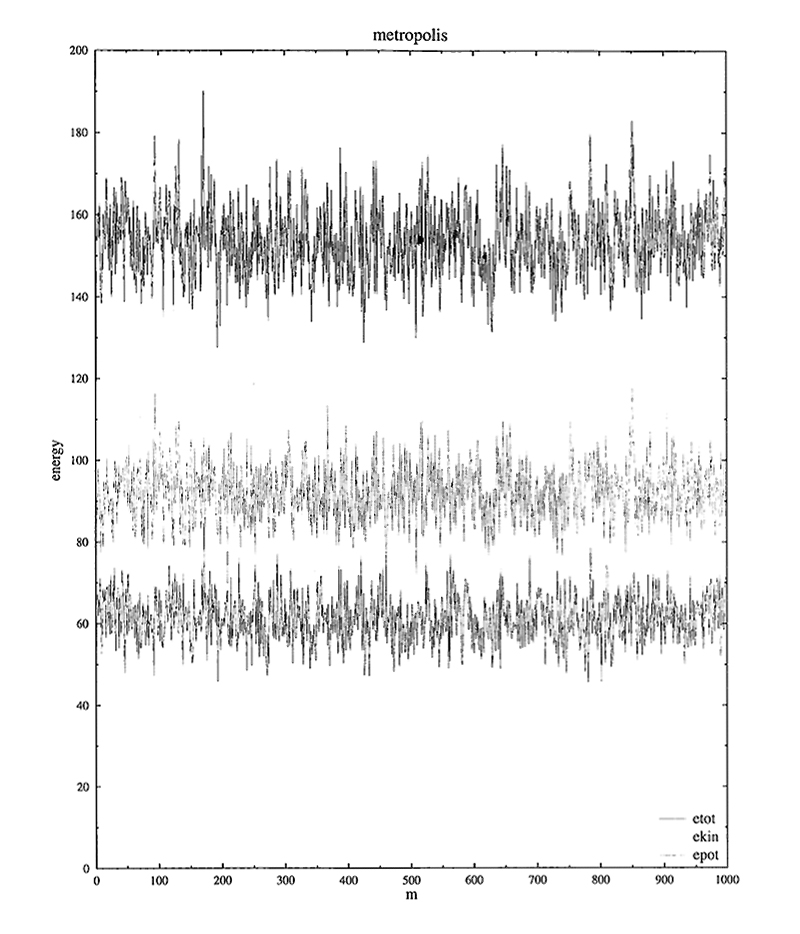
\includegraphics[width=190mm]{EnergyPlot.jpg}
\caption{Energy vs Sweep Count}
\label{overflow}
\end{figure}

\end{document}  